%\documentclass[a4paper,12pt]{article}

%\usepackage{graphics}
%\usepackage[pdftex]{graphicx}

%\begin{document}

\subsection{Topologie de l'Internet}
\par
Comme expliqu\'e pr\'ec\'edemment, Internet n'est pas un seul grand r\'eseau. Il s'agit en fait de l'interconnexion de plusieurs r\'eseaux ou syst\`emes autonomes (AS). Un syst\`eme autonome est un r\'eseau r\'egi par une administration et soumis \`a un ensemble de r\`egles de routage internes. Les AS sont reli\'es entre eux par diff\'erents types de liens. Ces liens peuvent \^etre de type:
\begin{description}
 \item[PEER : ] accord commercial \`a travers lequel les clients respectifs de deux AS peuvent communiquer entre eux sans que les AS ne doivent se payer la connexion,
 \item[P2C ou C2P : ] il s'agit d'un lien commercial \`a travers lequel un AS devient le client d'un autre afin d'y transmettre tout ou partie de son trafic.
\end{description}
\par
Au coeur de l'Internet, on trouve les op\'erateurs appel\'es \textit{Tier One} qui sont reli\'es deux \`a deux par des liens de type PEER au sein d'une structure en full-mesh aussi appel\'ee \textit{clique} en th\'eorie des graphes. Les \textit{Tier One} sont les grands op\'erateurs qui forment le coeur de l'Internet. Ils en sont en quelque sorte le ciment et les gardiens. 
\par
%Ils sont tous reli\'es deux \`a deux par des accords de type PEER, et ne peuvent pas se d\'econnecter. Meule nous a expliqué le contraire... Avec ses exemple sur Sprint, de plus tu l'a déjà dit pour la partie connexion en PEER
 Les \textit{Tier One} peuvent atteindre n'importe quelle destination sur Internet sans avoir \`a payer une seule connexion, puisqu'\`a plus ou moins haut niveau, tout AS est client potentiel d'un \textit{Tier One}. On retrouve parmis les \textit{Tier One} quelques grands noms des télécommunications (qui ne sont pas forcément des fournisseurs d'acc\`es) : Orange, Verizon Business, Sprint, AT\&T.
\par
Se relient \`a ces grands op\'erateurs d'autres AS qui peuvent eux-m\^eme \^etre reli\'es \`a d'autres et ainsi de suite. En outre, de fa\c con locale, on peut retrouver des full-mesh.
\par
Globalement, Internet a une structure connexe, c'est-\`a-dire que si l'on prend deux AS au hasard, il existe un chemin qui les relie. Il revient donc \`a chaque AS d'assurer la visibilit\'e de ses clients \`a travers le r\'eseau.
\par
En bout de cha\^ine, il y a des stubs. Ce sont des AS qui sont clients d'un ou plusieurs autres AS mais qui n'ont pas de client \`a eux. Quand un AS stub est reli\'e \`a un seul AS, on dit qu'il est \textit{monohom\'e}, si au contraire, il est le client de plusieurs autres AS en m\^eme temps, on dit alors qu'il est \textit{multi-hom\'e}. Le multi-homing permet de palier à la défaillance de l'un de ses fournisseurs d'accès.
\par
C'est pour cela que l'on dit que la topologie d'internet est hierarchique. C'est une sorte de pyramide avec à son sommet le \textit{Tier One} et à sa base les stubs.

\subsubsection{Repr\'esentation d'Internet}
\par
De fa\c con pratique, on peut repr\'esenter Internet comme un graphe o\`u les sommets sont les AS et les ar\^etes les liens entre les AS. La figure \ref{topologie} montre un exemple de cette repr\'esentation avec un coeur de l'Internet compos\'e de trois AS auxquels sont connect\'es d'autres AS. 
%On remarque que certain AS peuvent \^etre client aupr\`es de plusieurs AS en m\^eme temps. Cette m\'ethode est utile pour garantir un connectivit\'e m\^eme en cas de d\'efaillance d'une connection. Tu te répètes avec ce qu'il y au-dessus

\begin{figure}[ht]
\centering
 \fbox
 {
 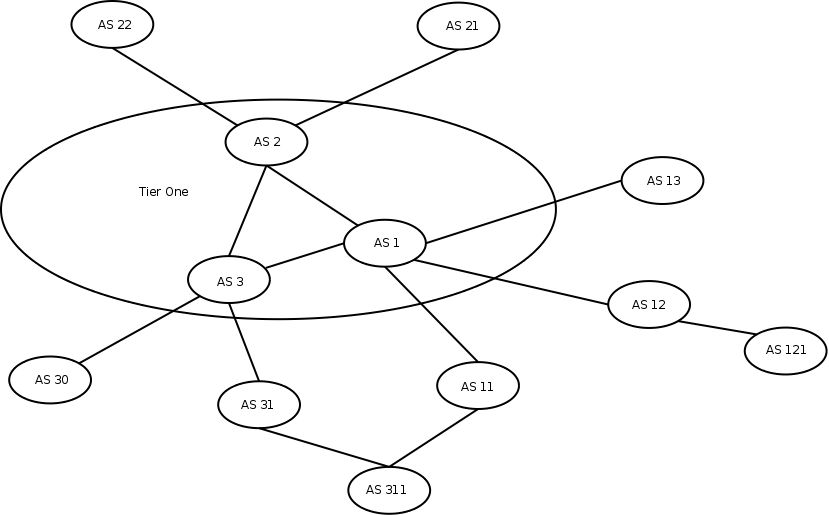
\includegraphics[width=16cm]{./schema/topologie_internet.png}
 }
  \caption{\label{topologie}Topologie d'Internet, exemple de repr\'esentation}
\end{figure}



%\end{document}
